%\documentclass{article}
%\documentclass[runningheads]{llncs}
%\documentclass[conference,onecolumn]{IEEEtran}
%\documentclass[preprint,12pt,authoryear]{elsarticle}
%\documentclass[preprint,1p  ,authoryear]{elsarticle}
\documentclass[preprint,1p]{elsarticle}

% Useful packages
% Language setting
% Replace `english' with e.g. `spanish' to change the document language
\usepackage[english]{babel}
\usepackage{amsmath}
\usepackage{amssymb}
\usepackage{graphicx}
%\usepackage{wrapfig}
%\usepackage[caption=false]{subfig}
% Define a new format for the figure index entry without the colon
\usepackage{caption}
%\captionsetup[table]{labelsep=space}
%\captionsetup{labelsep=space}
\usepackage{subcaption}

\usepackage[colorlinks=true, allcolors=blue]
{hyperref}
\usepackage{amsthm}
% If you use the hyperref package, please uncomment the following line
% to display URLs in blue roman font according to Springer's eBook style:
\renewcommand\UrlFont{\color{blue}\rmfamily}

%\usepackage{algorithm}
%\usepackage{arevmath}     % For math symbols
%\usepackage[noend]{algpseudocode}
\usepackage[linesnumbered,ruled,vlined]{algorithm2e}

% For multilined table cells
\usepackage{makecell}
\usepackage{tabularx}
\usepackage[table]{xcolor}

%%% Coloring the comment as blue
\newcommand\mycommfont[1]{\footnotesize\ttfamily\textcolor{blue}{#1}}
\SetCommentSty{mycommfont}

\SetKwInput{KwInput}{Input}                % Set the Input
\SetKwInput{KwOutput}{Output}              % set the Output
\newtheorem{theorem}{Theorem}
\newtheorem{lemma}[theorem]{Lemma}
%\renewcommand\qedsymbol{$\blacksquare$}

\DeclareMathOperator{\sha256}{sha256}
\DeclareMathOperator{\ThresholdOr}{ThresholdOr}

%\authorrunning{S. Dolev \and A. Fok \and M. Segal}
%\institute{Ben Gurion University, Beer Sheva, Israel}

%\date{February 2023}
\makeatletter
\newcommand{\vast}{\bBigg@{5}}

%\title{Waves Interference for Perfect Output VES  in Spite of Byzantine Participants}

% {\large\rm (Preliminary Version)}}

%%%%%%%%% 05012025
%\date{}
% \IEEEoverridecommandlockouts
% \IEEEpubid{\makebox[\columnwidth]{979-8-3503-9730-7/22/\$31.00~\copyright{}2022 IEEE \hfill}\hspace{\columnsep}\makebox[\columnwidth]{ }}
%\journal{Ad Hoc Networks}
\usepackage{tikz}
\usetikzlibrary{positioning, shapes.misc, arrows.meta}
% \usepackage{tikz}
% \usetikzlibrary{positioning, shapes.geometric, arrows.meta}

\tikzset{
  block/.style={rectangle, draw, minimum width=2.4cm, minimum height=1cm, align=center, font=\small},
  roundblock/.style={rounded rectangle, draw, minimum width=2.4cm, minimum height=1cm, align=center, font=\small},
  arrow/.style={->, thick},
}

\begin{document}

\begin{frontmatter}

\title{Quantum Perfect Output VES in Spite of Swarm Byzantine Participants}
% \author{

% \IEEEauthorblockN{Shlomi Dolev, {\it Fellow}, IEEE}
% \IEEEauthorblockA{\textit{Computer Science Department} \\
% \textit{Ben-Gurion University of the Negev}\\
% Beer-Sheva, Israel \\
% dolev@bgu.ac.il}
\author[first]{Shlomi Dolev}
\affiliation[first]{organization={Computer Science Department, Ben-Gurion University of the Negev},%Department and Organization
}
\affiliation[second]{organization={School of Electrical and Computer Engineering, Ben-Gurion University of the Negev},%Department and Organization
}
\author[second]{Alexander Fok}
\author[second]{Michael Segal}
% \and

% %\IEEEauthorblockN{Alexander Fok}
% %\IEEEauthorblockA{\textit{School of Electrical and Computer %Engineering} \\
% %\textit{Ben-Gurion University of the Negev}\\
% %Beer-Sheva, Israel \\
% %alexfok@post.bgu.ac.il}


% \IEEEauthorblockN{Alexander Fok \ \ \ \ \ \ \ \ Michael Segal, {\it Senior Member}, IEEE }
% \IEEEauthorblockA{\textit{School of Electrical and Computer Engineering} \\
% \textit{Ben-Gurion University of the Negev}\\
% Beer-Sheva, Israel \\
% alexfok@post.bgu.ac.il, segal@bgu.ac.il}
% }

% %\author{Shlomi Dolev, Alexander Fok, Michael Segal}
% %\authorrunning{S. Dolev \and A. Fok \and M. Segal}
% %\institute{Ben Gurion University, Beer Sheva, Israel}
% %\author{}
% \IEEEpeerreviewmaketitle
%%%%%%%%% 05012025

%%%%%%%%% 05012025
%\maketitle

% \author{Shlomi Dolev \and Alexander Fok \and Michael Segal}
% \authorrunning{S. Dolev \and A. Fok \and M. Segal}
% \institute{Ben Gurion University of the Negev, Beer Sheba, Israel}

% \maketitle % typeset the header of the contribution

\begin{abstract}
\noindent
\end{abstract}

\begin{keyword}
Quantum\sep Visual Secret Sharing \sep Swarm of UAVs \sep Visual Encryption Scheme \sep Byzantine adversaries \sep Perfect Output VES
\end{keyword}

\end{frontmatter}

\section{Introduction}
\label{chapter:intro}

\begin{figure}[ht]
\centering
\includegraphics[width=0.45\textwidth]{images/bloch_rbe_encryption_with_decryption.png}
\caption{Bloch sphere visualization of RBE encryption and decryption. The red vector represents the qubit state $|\psi\rangle = K_{\theta,\phi}|b\rangle$, while the green vector shows the result of decryption using $K_{\theta,\phi}^\dagger$, which restores the original basis state $|b\rangle$.}
\label{fig:bloch-rbe-decryption}
\end{figure}

% Known Visual Encryption Scheme (VES) encodes the secret image pixels into subpixel maps (shares) of size $m \times m$, where $m$ is a scheme parameter. The problem comes from the application where the swarm of Unmanned Aerial Vehicles (UAV) search for some target specified by an image.
% %\textcolor{blue}{
% The problem is defined as follows. A secret image is shared among a set of $n$ UAVs, which must collaboratively determine whether a candidate image matches the original, without reconstructing or revealing the secret image itself. This scenario is motivated by a practical application involving a swarm of UAVs engaged in a coordinated search mission, where the target is specified by a reference image known only to the system. The objective is to develop a solution that enables accurate image matching while preserving the confidentiality of the secret image, even in the presence of potentially compromised UAVs.
% %} % \textcolor{blue}
% The encoding of pixels typically relies on specific visual properties, such as transparency, as in \cite{naor1994visual} or light intensity, as in \cite{Jiao:20}.
% These subpixel maps consist of black and white pixels, as illustrated in Figure~\ref{fig:v2_VESPixelsEncoding}. 
% To reconstruct the original secret image, the shares are stacked together. If we put source of light under the stacked shares (created from pixel transparencies), the reconstructed image will look grey with darker or whiter pixels, namely, there will not be a totally white pixel. Naor and Shamir in \cite{naor1994visual} refer to this phenomenon as \textbf{the monotonicity problem}. It happens because the stacked subpixel maps represent different levels of grey - from very black to some level of grey. More precisely, stacked subpixel maps representing black pixels will have more than $k$ black subpixels in the same positions of $m \times m$ maps, and  stacked subpixel maps representing white pixels will have less than $k$ black subpixels in the same positions of $m \times m$ maps, as shown in Figure~\ref{fig:v2_VESPixelsEncoding}.
% Some existing VES schemes, including the original scheme by Naor and Shamir as described in \cite{naor1994visual}, can be extended to conceal the secret image. There are various methods to generate shares from the secret image, but all known methods produce grey scale shares that do not effectively hide the fact that there is secret communication. For instance, by using Naor and Shamir's proposed image concealing extension, innocent images of a dog and a cat can be used to hide an image of a house. 
% To achieve this, we create two shares - $D$ that represents the dog and $C$ that represents the cat. When $D$ and $C$ are stacked, they reveal $H$ - secret image of house. The problem here is that all the  aforementioned  images, are grey images. It includes shares $D$ and $C$, as well as the reconstructed image $H$. Using grey images exposes the presence of secret communication, necessitating additional protective measures that complicate implementation and can degrade image quality.
% The optical VES solution proposed in this work leverages a physical model of waves interference. The secret image reconstructed with the waves interference VES consists of pure white and black pixels, while preserving the computational efficiency of traditional VES methods. The waves interference VES is described in \ref{chapter:our_solution}.
% In section \ref{sec_model_analysis}, we show that the proposed VES scheme offers robust security. It is perfect information theoretical secure against honest and curious adversaries, while also withstanding attacks from active, Byzantine adversaries. The resilience against Byzantine adversaries provides the optical VES with a significant advantage in unstable environments such as UAV swarms.
% To the best of our knowledge, none of the existing VESs copes with active (Byzantine) adversaries. To disrupt the distributed pixel recovery decision, a Byzantine adversary needs to controls small part of swarm participants in the way it can affect their pixel maps.
% In section \ref{collaborative_secure_images_matching} we extend the waves inference VES to cope with Collaborative Secure Images Matching problem, described in paper \cite{10013507}. 


\section{Related Work}
\label{chapter:related_work}


% \subsection{Random Basis Encryption (RBE)}
% \label{sec:related_rbe}

% Random Basis Encryption (RBE), proposed by Bitan and Dolev~\cite{bitan2023randomlychooseangleimmense}, is a quantum homomorphic encryption scheme designed for classical data. Unlike the traditional Quantum One-Time Pad (QOTP), which encodes a bit using one of four Pauli-transformed qubit states, RBE selects from an immense continuum of possible bases. This design significantly improves security against adversaries capable of weak quantum measurements.

% In RBE, a classical bit $b \in \{0,1\}$ is encrypted as a qubit $\vert \psi_b \rangle$ using a unitary operator $K_{\theta, \phi}$ drawn from a random basis defined by two angles: $\theta \in [0, 2\pi]$ and $\phi \in \{\pm \frac{\pi}{2}\}$. The ciphertext is:
% \[
% \vert \psi_b \rangle = K_{\theta, \phi} \vert b \rangle.
% \]

% The decryption is performed using the Hermitian conjugate:
% \[
% \vert b \rangle = K_{\theta, \phi}^{\dagger} \vert \psi_b \rangle,
% \]
% followed by a standard basis measurement.

% The RBE scheme provides the following key properties:
% \begin{itemize}
%   \item \textbf{Information-theoretic (IT) security}: Measurements in an incorrect basis yield completely random outcomes.
%   \item \textbf{Perfect correctness}: Decryption always recovers the original bit with probability 1.
%   \item \textbf{Homomorphic gate support}: Operations like NOT and CNOT can be applied directly to encrypted qubits, enabling secure transformations without decrypting.
%   \item \textbf{Non-interactive evaluation}: The encryption keys are not needed during computation, unlike in QOTP-based schemes that require key updates.
%   \item \textbf{Weak measurement resilience}: Since the encoding basis is drawn from a large (potentially continuous) set, the adversary cannot perform effective inference without collapsing the state.
% \end{itemize}

% In the context of Visual Encryption Schemes (VES), RBE provides an elegant mechanism for encoding image pixels into qubits while enabling operations like pattern matching, pixel inversion, or entanglement without revealing the underlying image content. Its compactness and computation-agnostic nature make it particularly suitable for decentralized image encryption scenarios, such as those involving UAV swarms or collaborative matching in untrusted environments.

\subsection{Random Basis Encryption (RBE)}
\label{sec:related_rbe}

Random Basis Encryption (RBE), proposed by Bitan and Dolev~\cite{bitan2023randomlychooseangleimmense}, is an information-theoretically secure (IT-secure) quantum homomorphic encryption scheme tailored for classical data. It overcomes key limitations of the widely used Quantum One-Time Pad (QOTP), which only supports a small set of encryption keys (from the four Pauli gates) and requires interaction or key updates during evaluation.

In contrast, RBE leverages a continuously parameterized space of quantum bases, offering significantly higher entropy per bit and better protection against quantum side-channel attacks such as weak measurements.

\paragraph{Encryption.}
Given a classical bit $b \in \{0,1\}$, the encryption process selects a random basis defined by two angles:
\[
(\theta, \phi) \in [0, 2\pi] \times \left\{ \pm \frac{\pi}{2} \right\}.
\]

Using this basis, the dealer constructs a unitary operator:
\[
K_{\theta,\phi} = 
\begin{bmatrix}
\cos(\theta/2) & \sin(\theta/2) \\
e^{i\phi} \sin(\theta/2) & -e^{i\phi} \cos(\theta/2)
\end{bmatrix},
\]
and applies it to the computational basis state $|b\rangle$ to produce the ciphertext qubit:
\[
|\psi_b\rangle = K_{\theta,\phi} |b\rangle.
\]

\paragraph{Decryption.}
To decrypt, the inverse operator $K_{\theta,\phi}^\dagger$ is applied:
\[
K_{\theta,\phi}^\dagger |\psi_b\rangle = |b\rangle,
\]
followed by measurement in the computational basis.

\paragraph{Security.}
RBE is proven to be perfectly secure: for an adversary who does not know the basis $(\theta,\phi)$, any measurement of $|\psi_b\rangle$ yields a uniformly random bit, independent of $b$. This holds even when the adversary chooses the measurement basis arbitrarily. The scheme's security proof covers both classical and quantum adversaries, and is resilient against weak measurement attacks that might otherwise gain partial information in protocols like BB84 or QOTP-based schemes.

\paragraph{Homomorphic Evaluation.}
RBE supports non-interactive homomorphic evaluation of certain quantum gates:
\begin{itemize}
  \item \textbf{NOT:} Applies a logical flip to the encrypted bit.
  \item \textbf{CNOT:} Enables controlled operations when control is in the computational basis.
  \item \textbf{D gate:} Used to emulate Hadamard-like interference effects, especially useful in visual encryption and pattern-matching.
\end{itemize}

Importantly, these operations can be performed directly on the ciphertext without modifying the encryption key or requiring interaction with the sender.

This makes RBE particularly well-suited for distributed or swarm-based scenarios, such as UAVs evaluating candidate images, where qubits may be processed by untrusted nodes and later returned for trusted decryption.


\begin{figure}[ht]
\centering
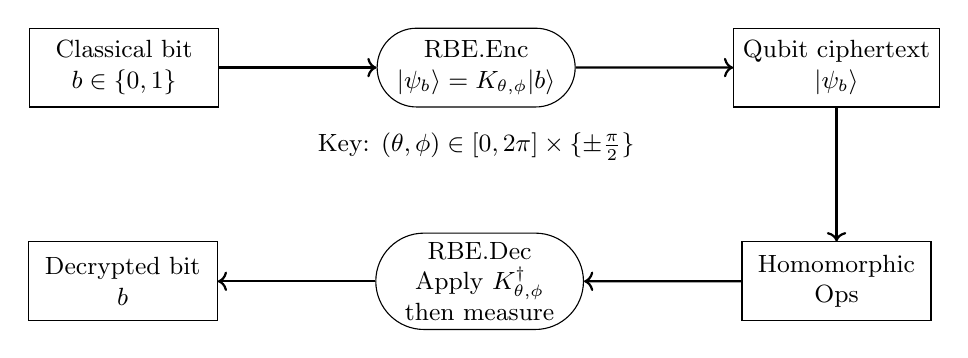
\begin{tikzpicture}[node distance=1.7cm and 2cm]

  % Nodes
  \node[block] (bit) {Classical bit\\$b \in \{0,1\}$};
  \node[roundblock, right=of bit] (rbeenc) {RBE.Enc\\$\vert\psi_b\rangle = K_{\theta,\phi} \vert b\rangle$};
  \node[block, right=of rbeenc] (cipher) {Qubit ciphertext\\$\vert\psi_b\rangle$};
%  \node[block, below=of cipher] (gate) {Homomorphic gate\\(e.g., NOT, CNOT)};
% Replace the existing node label:
%  \node[block, below=of cipher] (gate) {Homomorphic or In-transit\\(e.g., NOT, CNOT, $\otimes D$)};
  \node[block, below=of cipher] (gate) {Homomorphic \\Ops};
  \node[roundblock, left=of gate] (rbedec) {RBE.Dec\\Apply $K_{\theta,\phi}^\dagger$\\then measure};
  \node[block, left=of rbedec] (output) {Decrypted bit\\$b$};
%  \node[block, anchor=west, yshift=-3.4cm] (output) at (bit.west) {Decrypted bit\\$b$};
%  \node[block, anchor=west, yshift=-3.4cm] (output) at (bit.west) {Decrypted bit\\$b$};


% Optional note under the flow:
%\node[below=0.2cm of gate, font=\small, align=center] {Operations optional;\\may remain in superposition until dealer measures};

  % Arrows
  \draw[arrow] (bit) -- (rbeenc);
  \draw[arrow] (rbeenc) -- (cipher);
  \draw[arrow] (cipher) -- (gate);
  \draw[arrow] (gate) -- (rbedec);
  \draw[arrow] (rbedec) -- (output);

  % Optional key info
  \node[below=0.2cm of rbeenc, font=\small] (keyinfo) {Key: $(\theta,\phi) \in [0,2\pi] \times \{\pm \frac{\pi}{2}\}$};

\end{tikzpicture}
\caption{RBE Encryption, Homomorphic Evaluation, and Decryption Flow}
\label{fig:rbe-diagram}
\end{figure}

\section{Our Solution}
\label{chapter:our_solution}

In this section, we present our novel Quantum Visual Encryption Scheme (VES), designed to overcome the limitations of existing methods. Traditional VES techniques often exhibit suboptimal contrast and limited resilience against Byzantine adversaries. Our approach leverages quantum computation to enhance both security and image quality. In particular, we employ the quantum gate $D$, as also utilized by researchers in \cite{bitan2023randomlychooseangleimmense}. Here is an example of $D$ operation:
\begin{equation}
\underbrace{QT[i]}_{\text{Pixel qubit}}
\ \otimes\ 
\underbrace{D}_{\text{Quantum gate}}
\quad=\quad
\begin{bmatrix}
q_{0} \\[0.2em]
q_{1}
\end{bmatrix}
\ \otimes\
\begin{bmatrix}
d_{00} & d_{01} \\[0.2em]
d_{10} & d_{11}
\end{bmatrix}
\quad=\quad
\begin{bmatrix}
q_{0} d_{00} & q_{0} d_{01} \\[0.2em]
q_{0} d_{10} & q_{0} d_{11} \\[0.5em]
q_{1} d_{00} & q_{1} d_{01} \\[0.2em]
q_{1} d_{10} & q_{1} d_{11}
\end{bmatrix}
\end{equation}

Let $T$ denote the secret image and $QT$ its quantum encoding. The $i$-th pixel of $T$ is represented as $T[i]$, and its corresponding qubit in $QT$ is $QT[i]$.

\paragraph{Encoding phase}
The dealer first encodes each pixel $T[i]$ into a qubit by applying the Hadamard gate, resulting in $QT[i]$ being placed in a superposition state. Subsequently, the dealer randomly distributes a subset of the qubits to $N$ participants. Each participant receives approximately $L/N$ qubits, where $L$ is the total number of pixels in the image.

A random basis $B$ is used for the encoding process and for generating the superposition states. This basis is known only to the dealer and remains secret from the participants. Importantly, the state of each pixel (black or white) is unknown to the participants. Determining the state requires measuring the qubit, which collapses its superposition.

\paragraph{Recovery phase}
Image recovery is straightforward: participants transmit their qubits back to the dealer, who measures them in the correct basis $B$, thereby revealing the original pixel states.

%]\footnote{The images used in this study are sourced from an online image database~\cite{online_image_database}.}.

%\subsection{Quantum Perfect Output Visual Encryption Scheme}


% Similarly to the existing VES schemes, Waves Interference based VES scheme encodes the secret image to two (or more) shares that look as random pixels collection, as shown in Figure \ref{fig:ves_optical_model}
% \begin{figure}[h!]
%     \centering
%     \includegraphics[width=0.6\textwidth,keepaspectratio]
% %    \includegraphics[width=\textwidth,keepaspectratio]
% {images/BWVES_model3.png}
%     \caption{VES Optical Model.}
%     \label{fig:ves_optical_model}
% \end{figure}
% The secret image can be recovered from the shares later.
% Our optical solution leverages wave interference to achieve a Visual Encryption Scheme that produces perfect images composed of pure black and white pixels.

\subsection{RBE-based Quantum Visual Encryption Sketch}
\label{sec:rbe_ves_sketch}

\paragraph{Use of RBE in Visual Encryption Schemes (VES).}
In VES settings, where images are encoded and distributed as quantum states (e.g., pixel-to-qubit mappings), RBE provides a natural building block:
\begin{itemize}
  \item Each pixel is encrypted independently using a fresh random basis, ensuring that partial leakage from one pixel provides no information about others.
  \item No pixel value is revealed until the ciphertext qubit is decrypted and measured using the correct key.
  \item Secure transformations (e.g., contrast inversion, pixel masking, feature matching) can be applied homomorphically without revealing the underlying image.
\end{itemize}


To illustrate how the RBE mechanism integrates into a Quantum Visual Encryption Scheme (VES), we provide a high-level system design that outlines the encoding, transformation, and decoding phases.

In this scheme, each pixel of the secret image is encoded as a qubit using the Random Basis Encryption (RBE) scheme \cite{bitan2023randomlychooseangleimmense}, which offers perfect information-theoretic security. The key idea is to encrypt each classical bit (black or white pixel) into a qubit using a unique and secret rotation basis.

Let $T \in \{0,1\}^{m \times n}$ be a binary image (black-and-white), and let $QT$ denote its quantum representation. Each pixel $T[i]$ is mapped to a qubit $QT[i] = \vert \psi_i \rangle$ using the encryption operator $K_{\theta_i, \phi_i}$ as follows:
\[
\vert \psi_i \rangle = K_{\theta_i, \phi_i} \vert T[i] \rangle,
\]
where $(\theta_i, \phi_i)$ is randomly drawn from $[0, 2\pi] \times \left\{\pm \frac{\pi}{2} \right\}$.

These qubits are distributed securely and may optionally undergo homomorphic operations (e.g., NOT or CNOT) by untrusted servers, without revealing their contents. Decryption is performed by applying $K_{\theta_i, \phi_i}^\dagger$ and measuring in the computational basis.

Figure~\ref{fig:rbe-ves-design} illustrates the full data flow.

\begin{figure}[ht]
\centering
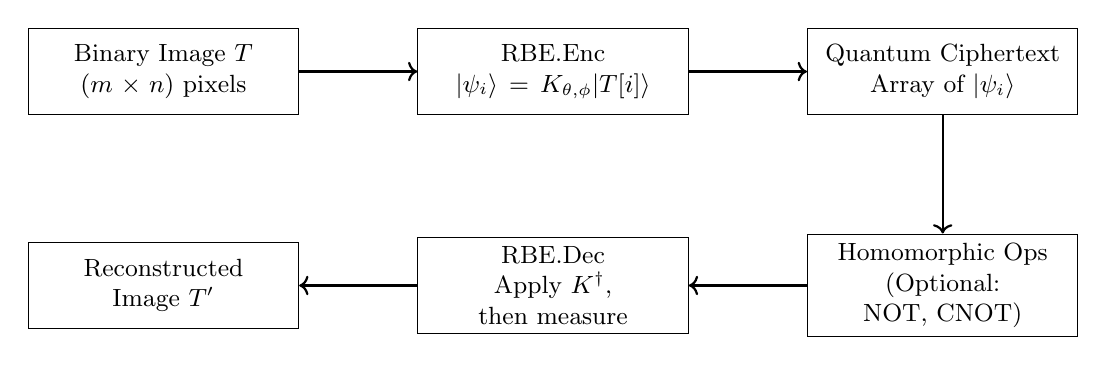
\begin{tikzpicture}[node distance=1.6cm and 1.5cm, font=\small]
  \tikzset{block/.style={rectangle, draw, minimum height=1.1cm, text width=3.2cm, align=center}}
  \tikzset{arrow/.style={->, thick}}

  \node[block] (input) {Binary Image $T$\\$(m \times n)$ pixels};
  \node[block, right=of input] (rbe) {RBE.Enc\\$\vert\psi_i\rangle = K_{\theta,\phi} \vert T[i]\rangle$};
  \node[block, right=of rbe] (cipher) {Quantum Ciphertext\\Array of $\vert \psi_i \rangle$};

  \node[block, below=1.5cm of cipher] (homomorphic) {Homomorphic Ops\\(Optional: NOT, CNOT)};
  \node[block, left=of homomorphic] (decrypt) {RBE.Dec\\Apply $K^\dagger$, then measure};
  \node[block, left=of decrypt] (output) {Reconstructed Image $T'$};

  \draw[arrow] (input) -- (rbe);
  \draw[arrow] (rbe) -- (cipher);
  \draw[arrow] (cipher) -- (homomorphic);
  \draw[arrow] (homomorphic) -- (decrypt);
  \draw[arrow] (decrypt) -- (output);
\end{tikzpicture}
\caption{Quantum VES design sketch using RBE as the encryption mechanism. Each pixel is encrypted into a qubit using a secret random basis, enabling secure storage, homomorphic processing, and accurate reconstruction.}
\label{fig:rbe-ves-design}
\end{figure}

\subsection{Multi-Participant Quantum VES with RBE}
\label{sec:rbe_multiuser_ves}

We extend the RBE-based quantum visual encryption scheme to support collaborative reconstruction and secure image matching across multiple distributed participants, such as UAV swarm nodes.

In this setting, a central dealer prepares the quantum-encoded image by encrypting each pixel $T[i]$ into a qubit $QT[i] = K_{\theta_i,\phi_i} \vert T[i] \rangle$ using the Random Basis Encryption (RBE) method~\cite{bitan2023randomlychooseangleimmense}. The encryption keys $(\theta_i, \phi_i)$ remain secret and are known only to the dealer.

Each qubit $QT[i]$ is then distributed among $N$ participants. The scheme supports two operational modes:

\begin{itemize}
    \item \textbf{Collaborative Reconstruction}: Participants return their qubits to the dealer. Once $d \leq N$ correct shares are received, the dealer measures them in the correct basis to reconstruct the pixel values. The threshold $d$ ensures robustness against Byzantine adversaries.
    \item \textbf{Secure Pixel Matching}: Participants perform homomorphic transformations on encrypted qubits (e.g., via $\otimes D$ for comparison), based on observed candidate pixels, without learning the original data. Transformed qubits are returned to the dealer for evaluation.
\end{itemize}

This design achieves perfect information-theoretic security, non-interactivity, and resilience to active adversaries. Additionally, the RBE encoding inherently prevents weak measurement-based leakage, as adversaries lack the basis information required to extract signal without collapsing the state.


\begin{figure}[ht]
\centering
\resizebox{\linewidth}{!}{
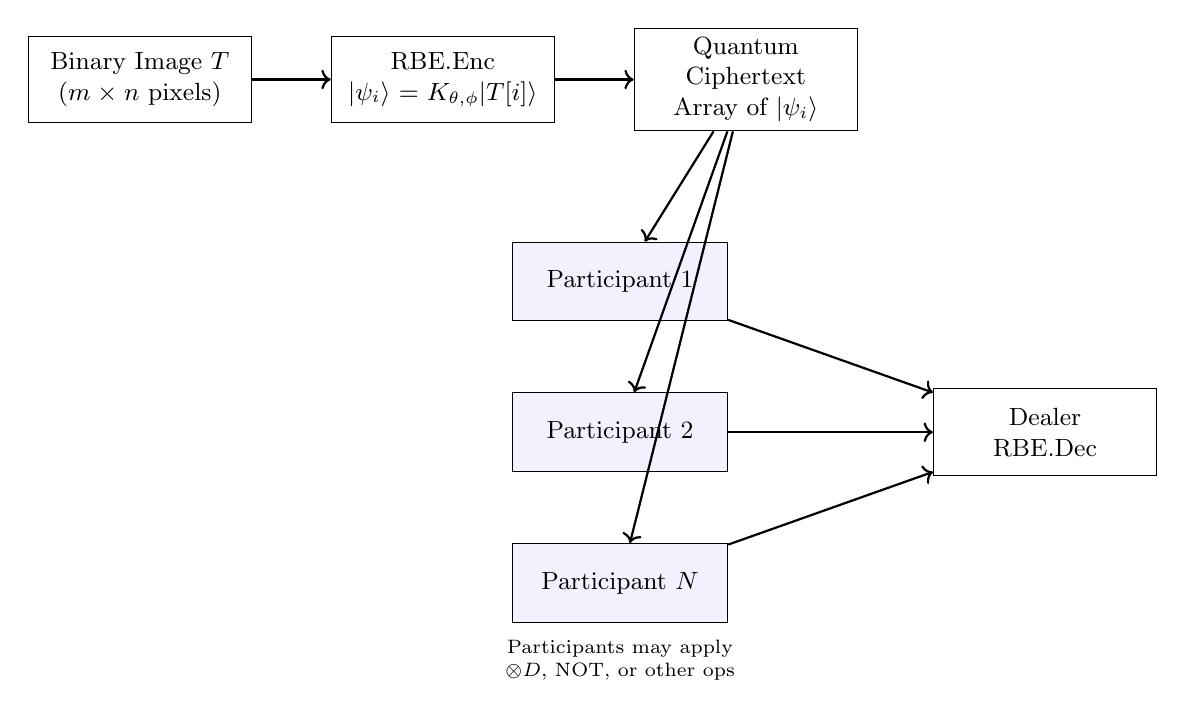
\begin{tikzpicture}[node distance=1.6cm and 1.0cm, font=\small]
  \tikzset{
    block/.style={rectangle, draw, minimum height=1.1cm, text width=2.6cm, align=center},
    participant/.style={rectangle, draw, minimum height=1cm, text width=2.5cm, align=center, fill=blue!5},
    arrow/.style={->, thick},
  }

  \node[block] (input) {Binary Image $T$\\($m \times n$ pixels)};
  \node[block, right=of input] (rbe) {RBE.Enc\\$\vert\psi_i\rangle = K_{\theta,\phi} \vert T[i]\rangle$};
  \node[block, right=of rbe] (cipher) {Quantum Ciphertext\\Array of $\vert \psi_i \rangle$};

  \node[participant, below left=1.4cm and -1.2cm of cipher] (p1) {Participant 1};
  \node[participant, below=0.9cm of p1] (p2) {Participant 2};
  \node[participant, below=0.9cm of p2] (p3) {Participant $N$};

  \node[block, right=2.6cm of p2] (dealer) {Dealer\\RBE.Dec};

  \draw[arrow] (input) -- (rbe);
  \draw[arrow] (rbe) -- (cipher);
  \draw[arrow] (cipher) -- (p1);
  \draw[arrow] (cipher) -- (p2);
  \draw[arrow] (cipher) -- (p3);
  \draw[arrow] (p1) -- (dealer);
  \draw[arrow] (p2) -- (dealer);
  \draw[arrow] (p3) -- (dealer);

  \node[below=0.1cm of p3, font=\scriptsize, align=center] (note) {Participants may apply\\$\otimes D$, NOT, or other ops};
\end{tikzpicture}
}
\caption{Quantum Visual Encryption Scheme with RBE for multiple participants.}
\label{fig:rbe-ves-multiparty}
\end{figure}

\subsection{Quantum VES with Secure Image Matching}
\label{sec:q_ves_sec_image_match}

We extend the RBE-based quantum visual encryption scheme to support collaborative reconstruction and secure image matching across multiple distributed participants, such as UAV swarm nodes.

In this setting, a central dealer prepares the quantum-encoded image by encrypting each pixel $T[i]$ into a qubit $QT[i] = K_{\theta_i,\phi_i} \vert T[i] \rangle$ using the Random Basis Encryption (RBE) method~\cite{bitan2023randomlychooseangleimmense}. The encryption keys $(\theta_i, \phi_i)$ remain secret and are known only to the dealer.

Each qubit $QT[i]$ is then distributed among $N$ participants. The scheme supports two operational modes:

\begin{itemize}
    \item \textbf{Collaborative Reconstruction}: Participants return their encoded qubits to the dealer. Once $d \leq N$ correct shares are received, the dealer measures them in the correct basis to reconstruct the pixel values. The threshold $d$ ensures robustness against Byzantine adversaries.
    \item \textbf{Secure Pixel Matching}: Each participant locally observes a candidate image pixel $C[i] \in \{0,1\}$. If $C[i] = 1$, they apply a controlled quantum gate (e.g., CNOT) on the encoded qubit $QT[i]$, without knowing its content. The modified qubit is returned to the dealer, who evaluates the match using the decryption key.
\end{itemize}

This design achieves perfect information-theoretic security, non-interactivity, and resilience to active adversaries. Additionally, the RBE encoding inherently prevents weak measurement-based leakage, as adversaries lack the basis information required to extract signal without collapsing the state.

\begin{figure}[ht]
\centering
\resizebox{\linewidth}{!}{
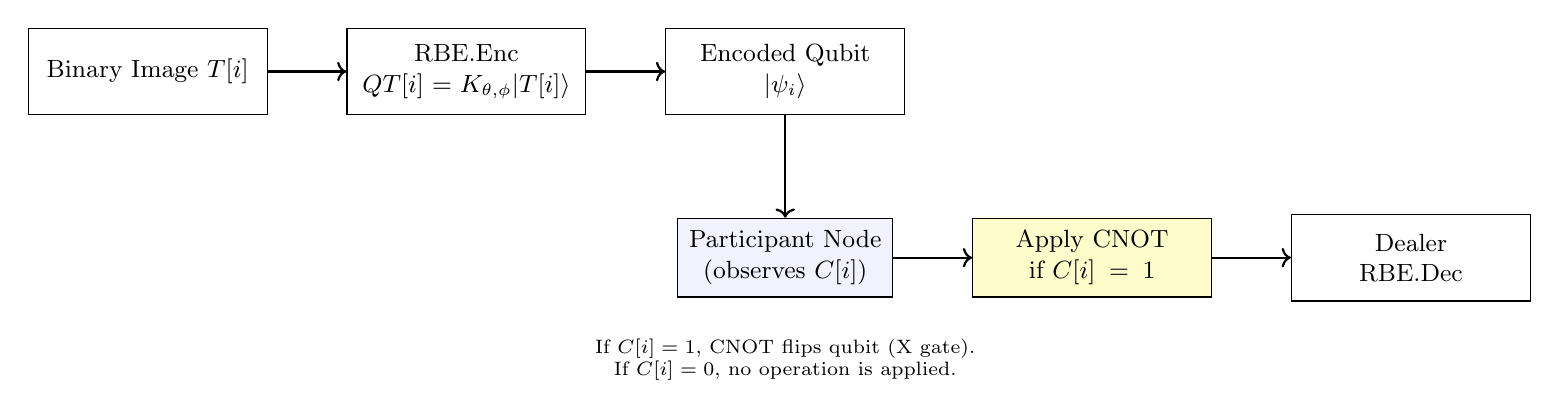
\begin{tikzpicture}[node distance=1.6cm and 1.0cm, font=\small]
  \tikzset{
    block/.style={rectangle, draw, minimum height=1.1cm, text width=2.8cm, align=center},
    participant/.style={rectangle, draw, minimum height=1cm, text width=2.5cm, align=center, fill=blue!5},
    operation/.style={rectangle, draw, minimum height=1cm, text width=2.8cm, align=center, fill=yellow!20},
    arrow/.style={->, thick},
  }

  % Nodes
  \node[block] (input) {Binary Image $T[i]$};
  \node[block, right=of input] (rbe) {RBE.Enc\\$QT[i] = K_{\theta,\phi}|T[i]\rangle$};
  \node[block, right=of rbe] (cipher) {Encoded Qubit\\$|\psi_i\rangle$};
  \node[participant, below=1.3cm of cipher] (p1) {Participant Node\\(observes $C[i]$)};
  \node[operation, right=of p1] (cnot) {Apply CNOT\\if $C[i] = 1$};
  \node[block, right=of cnot] (dealer) {Dealer\\RBE.Dec};

  % Arrows
  \draw[arrow] (input) -- (rbe);
  \draw[arrow] (rbe) -- (cipher);
  \draw[arrow] (cipher) -- (p1);
  \draw[arrow] (p1) -- (cnot);
  \draw[arrow] (cnot) -- (dealer);

  % Note
  \node[below=0.4cm of p1, font=\scriptsize, align=center] (note) {
    If $C[i]=1$, CNOT flips qubit (X gate).\\
    If $C[i]=0$, no operation is applied.
  };

\end{tikzpicture}
}
\caption{Quantum VES with RBE encryption and homomorphic CNOT matching. The participant uses its classical candidate pixel $C[i]$ to optionally apply a CNOT to the encrypted qubit $QT[i]$ before returning it to the dealer.}
\label{fig:qves-cnot-tikz}
\end{figure}

% \begin{figure}[ht]
% \centering
% \includegraphics[width=0.95\linewidth]{images/quantum_ves_cnot_diagram.png}
% \caption{
% Quantum VES scheme with RBE encryption and CNOT-based homomorphic matching.
% Each image pixel $T[i]$ is encrypted into a qubit $QT[i] = K_{\theta,\phi}|T[i]\rangle$.
% Participants observe candidate pixels $C[i] \in \{0,1\}$ and apply a CNOT gate to $QT[i]$ if and only if $C[i]=1$.
% The resulting qubits are sent back to the dealer, who decrypts them and evaluates whether $T[i] = C[i]$.
% }
% \label{fig:qves-cnot}
% \end{figure}

\begin{table}[ht]
\centering
\renewcommand{\arraystretch}{1.4}
\begin{tabular}{|p{2.5cm}|p{2.1cm}|p{2.2cm}|p{2.7cm}|p{2.3cm}|}
\hline
\makecell{\textbf{Encrypted}\\\textbf{Pixel} ($QT[i]$)} &
\makecell{\textbf{Candidate}\\\textbf{Pixel} $C[i]$} &
\makecell{\textbf{Operation}\\(if $C[i] = 1$)} &
\makecell{\textbf{Transformed}\\\textbf{Qubit}} &
\makecell{\textbf{Match}\\\textbf{Result}} \\
\hline
$\vert 0 \rangle$ & $0$ & None & $\vert 0 \rangle$ & Match \\
$\vert 0 \rangle$ & $1$ & CNOT & $\vert 0 \rangle$ & Mismatch \\
$\vert 1 \rangle$ & $0$ & None & $\vert 1 \rangle$ & Mismatch \\
$\vert 1 \rangle$ & $1$ & CNOT & $\vert 0 \rangle$ & Match \\
\hline
\end{tabular}
\caption{Truth table for secure image matching using CNOT on encrypted qubit $QT[i]$. A CNOT is applied only when the classical candidate pixel $C[i] = 1$. The dealer decrypts the transformed qubit and determines whether $T[i] = C[i]$.}
\label{tab:cnot-matching}
\end{table}

% 3 types of participants:
% A - Keep encrypted qubits
% B - Keep RBE encryption keys
% C - Acquire candidate images C[i]

% 3 flows:
% Encryption
% Dealer: Binary image -> RBE.Enc -> Encoded Qubit to A
%     -> RBE keys to B

% Recovery
% A: Encoded Qubit to Dealer
% B: RBE keys to Dealer RBE.Dec -> Binary Image

% Matching
% C: Acquire candidate image C[i] and pass it to B
% B: RBE.Dec(C[i]) AND CNOT -> Transformed Qubit

\subsection{Quantum VES with Distributed Roles and Secure Matching Old}
\label{sec:qves_distributed_roles_old}

We refine the RBE-based quantum visual encryption scheme by introducing three distinct participant roles to improve modularity, reduce risk, and separate sensitive quantum resources:

\begin{itemize}
  \item \textbf{Type A}: Receives and stores the quantum-encoded qubits $QT[i] = K_{\theta_i,\phi_i} |T[i]\rangle$ for each pixel.
  \item \textbf{Type B}: Receives and retains the RBE encryption keys $(\theta_i, \phi_i)$ and performs decryption operations.
  \item \textbf{Type C}: Acquires candidate image pixels $C[i]$ and forwards them to B for comparison.
\end{itemize}

The system operates in three phases:

\paragraph{Encryption} The dealer encrypts each pixel $T[i]$ using RBE:
\[
QT[i] = K_{\theta_i,\phi_i} |T[i]\rangle
\]
Then:
- $QT[i]$ is sent to participant A.
- $(\theta_i, \phi_i)$ are sent to participant B.

\paragraph{Recovery} Participants A and B collaboratively reconstruct the original image:
- A sends the stored qubits $QT[i]$ to the dealer.
- B sends the corresponding decryption keys.
- The dealer performs RBE.Dec to recover $T[i]$.

\paragraph{Matching} Participant C acquires a candidate image $C[i]$ and sends it to B:
- B applies a **conditional CNOT** operation on the decrypted state if $C[i] = 1$:
\[
QT'_i = \text{CNOT}(K_{\theta_i,\phi_i}^{\dagger} QT[i]) \quad \text{if } C[i] = 1
\]
- The resulting transformed qubit is returned to the dealer for evaluation.

\begin{figure}[ht]
\centering
\resizebox{\linewidth}{!}{
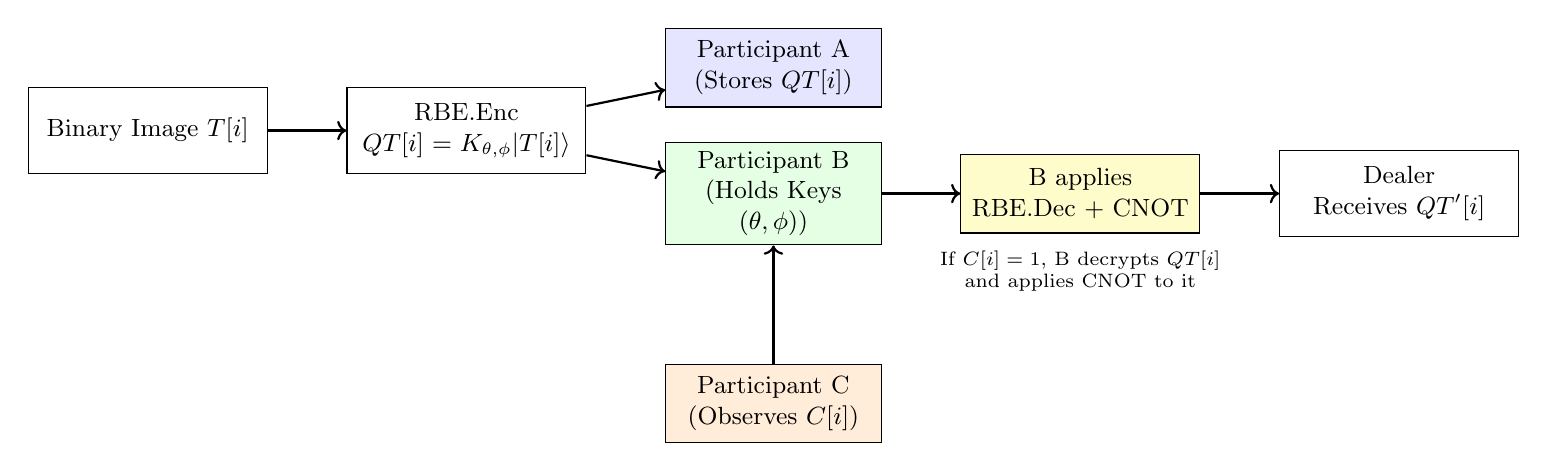
\begin{tikzpicture}[node distance=1.6cm and 1.0cm, font=\small]
  \tikzset{
    block/.style={rectangle, draw, minimum height=1.1cm, text width=2.8cm, align=center},
    participantA/.style={rectangle, draw, minimum height=1cm, text width=2.5cm, align=center, fill=blue!10},
    participantB/.style={rectangle, draw, minimum height=1cm, text width=2.5cm, align=center, fill=green!10},
    participantC/.style={rectangle, draw, minimum height=1cm, text width=2.5cm, align=center, fill=orange!15},
    operation/.style={rectangle, draw, minimum height=1cm, text width=2.8cm, align=center, fill=yellow!20},
    arrow/.style={->, thick},
  }

  % Encryption flow
  \node[block] (input) {Binary Image $T[i]$};
  \node[block, right=of input] (rbe) {RBE.Enc\\$QT[i] = K_{\theta,\phi}|T[i]\rangle$};
  \node[participantA, right=of rbe, yshift=0.8cm] (a) {Participant A\\(Stores $QT[i]$)};
  \node[participantB, right=of rbe, yshift=-0.8cm] (b) {Participant B\\(Holds Keys $(\theta, \phi)$)};
  
  % Matching
  \node[participantC, below=1.5cm of b] (c) {Participant C\\(Observes $C[i]$)};
  \node[operation, right=of b] (cnot) {B applies\\RBE.Dec + CNOT};
  \node[block, right=of cnot] (dealer) {Dealer\\Receives $QT'[i]$};

  % Arrows
  \draw[arrow] (input) -- (rbe);
  \draw[arrow] (rbe) -- (a);
  \draw[arrow] (rbe) -- (b);
  \draw[arrow] (c) -- (b);
  \draw[arrow] (b) -- (cnot);
  %\draw[arrow] (a) |- ([yshift=0.5cm]dealer.west);
  \draw[arrow] (cnot) -- (dealer);

  % Labels
  \node[below=0.1cm of cnot, font=\scriptsize, align=center] {
    If $C[i] = 1$, B decrypts $QT[i]$\\and applies CNOT to it
  };

\end{tikzpicture}
}
\caption{Quantum VES with separated roles: A stores quantum ciphertext, B holds encryption keys and performs decryption/matching, and C acquires classical candidate image pixels $C[i]$.}
\label{fig:qves-role-separation}
\end{figure}

\begin{table}[ht]
\centering
\renewcommand{\arraystretch}{1.4}
\begin{tabular}{|c|c|c|c|c|}
\hline
\makecell{\textbf{Original}\\\textbf{Pixel} $T[i]$} &
\makecell{\textbf{Candidate}\\\textbf{Pixel} $C[i]$} &
\makecell{\textbf{B decrypts}\\and applies CNOT} &
\makecell{\textbf{Transformed}\\\textbf{Qubit}} &
\makecell{\textbf{Match}\\\textbf{Result}} \\
\hline
$|0\rangle$ & $0$ & No & $|0\rangle$ & Match \\
$|0\rangle$ & $1$ & Yes & $|0\rangle$ & Mismatch \\
$|1\rangle$ & $0$ & No & $|1\rangle$ & Mismatch \\
$|1\rangle$ & $1$ & Yes & $|0\rangle$ & Match \\
\hline
\end{tabular}
\caption{Matching logic performed by participant B using RBE decryption and conditional CNOT. The dealer makes match decision based on all participants B partial results.}
\label{tab:cnot-truth-table-roles}
\end{table}


% Change the matching flow as follows:
% Participants order should be: A, C, B
% A passes to C QT[i]
% C applies CNOT on QT[i], given C[i]
% C passes CNOT result to B
% B applies RBE.Dec on it.
% B concludes match decision: If it 0, C[i] matches QT[i]
\newpage
\subsection{Quantum VES with Distributed Roles and Secure Matching}
\label{sec:qves_distributed_roles}

We refine the RBE-based quantum visual encryption scheme by introducing three distinct participant roles to improve modularity, reduce risk, and separate sensitive quantum resources:

\begin{itemize}
  \item \textbf{Type A}: Receives and stores the quantum-encoded qubits $QT[i] = K_{\theta_i,\phi_i} |T[i]\rangle$ for each pixel.
  \item \textbf{Type B}: Receives and retains the RBE encryption keys $(\theta_i, \phi_i)$ and performs final decryption and match decision.
  \item \textbf{Type C}: Acquires candidate image pixels $C[i]$ and homomorphically processes encrypted qubits.
\end{itemize}

The system operates in three phases:

\paragraph{Encryption} The dealer encrypts each pixel $T[i]$ using RBE:
\[
QT[i] = K_{\theta_i,\phi_i} |T[i]\rangle
\]
Then:
- $QT[i]$ is sent to participant A.
- $(\theta_i, \phi_i)$ are sent to participant B.

\paragraph{Recovery} Participants A and B collaboratively reconstruct the original image:
- A sends the stored qubits $QT[i]$ to the dealer.
- B sends the corresponding decryption keys.
- The dealer performs RBE.Dec to recover $T[i]$.

\paragraph{Matching} The process is securely distributed:
- A sends $QT[i]$ to C.
- C applies a **CNOT gate** to $QT[i]$ if $C[i] = 1$, and forwards the result to B.
- B performs RBE.Dec to retrieve the classical bit and concludes:
  \[
  \text{Match if } RBE.Dec(QT'[i]) = 0
  \]
In other words, if the decrypted qubit after CNOT results in $|0\rangle$, then the candidate pixel $C[i]$ matches the original pixel $T[i]$.

\begin{figure}[ht]
\centering
\resizebox{\linewidth}{!}{
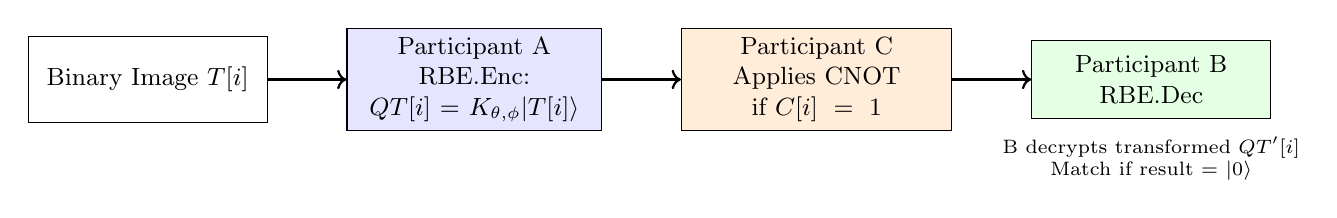
\begin{tikzpicture}[node distance=1.6cm and 1.0cm, font=\small]
  \tikzset{
    block/.style={rectangle, draw, minimum height=1.1cm, text width=2.8cm, align=center},
    participantA/.style={rectangle, draw, minimum height=1cm, text width=3.0cm, align=center, fill=blue!10},
    participantB/.style={rectangle, draw, minimum height=1cm, text width=2.8cm, align=center, fill=green!10},
    participantC/.style={rectangle, draw, minimum height=1cm, text width=3.2cm, align=center, fill=orange!15},
    arrow/.style={->, thick},
  }

  % Encryption flow
  \node[block] (input) {Binary Image $T[i]$};
  \node[participantA, right=of input] (a) {Participant A\\RBE.Enc:\\ $QT[i] = K_{\theta,\phi}|T[i]\rangle$};
  \node[participantC, right=of a] (c) {Participant C\\Applies CNOT if $C[i] = 1$};
  \node[participantB, right=of c] (b) {Participant B\\RBE.Dec};

  % Arrows
  \draw[arrow] (input) -- (a);
  \draw[arrow] (a) -- (c);
  \draw[arrow] (c) -- (b);

  % Label below B
  \node[below=0.1cm of b, font=\scriptsize, align=center] {
    B decrypts transformed $QT'[i]$\\
    Match if result = $|0\rangle$
  };

\end{tikzpicture}
}
\caption{Quantum VES with role separation: A encrypts and stores quantum pixels, C uses classical input $C[i]$ to apply CNOT, and B decrypts to determine match.}
\label{fig:qves-flow-enc-by-A}
\end{figure}

\begin{table}[ht]
\centering
\renewcommand{\arraystretch}{1.4}
\begin{tabular}{|c|c|c|c|c|}
\hline
\makecell{\textbf{Original}\\\textbf{Pixel} $T[i]$} &
\makecell{\textbf{Candidate}\\\textbf{Pixel} $C[i]$} &
\makecell{\textbf{C applies}\\CNOT on $QT[i]$} &
\makecell{\textbf{B decrypts}\\$QT'[i]$} &
\makecell{\textbf{Match}\\\textbf{Decision}} \\
\hline
$|0\rangle$ & $0$ & No & $|0\rangle$ & Match \\
$|0\rangle$ & $1$ & Yes & $|0\rangle$ & Mismatch \\
$|1\rangle$ & $0$ & No & $|1\rangle$ & Mismatch \\
$|1\rangle$ & $1$ & Yes & $|0\rangle$ & Match \\
\hline
\end{tabular}
\caption{Updated secure matching protocol: C applies CNOT conditioned on $C[i]$; B decrypts and concludes a match if the result is $|0\rangle$.}
\label{tab:cnot-truth-table-updated}
\end{table}



\subsection{Distributed Quantum VES with Role-Separated Matching}
\label{sec:qves_role_separated}

We introduce a distributed variant of the Random Basis Encryption (RBE) based quantum visual encryption scheme. In this design, roles are separated among three types of participants to support modularity, reduce attack surface, and enable secure matching without centralized decryption:

\begin{itemize}
  \item \textbf{Participant A}: Generates and stores quantum-encoded qubits $QT[i] = K_{\theta_i,\phi_i} |T[i]\rangle$.
  \item \textbf{Participant C}: Acquires candidate image pixels $C[i]$ and applies a controlled operation (CNOT) based on the pixel value.
  \item \textbf{Participant B}: Holds RBE keys $(\theta_i, \phi_i)$ and performs decryption to conclude match decisions.
\end{itemize}

\paragraph{Matching Flow} The protocol operates as follows:
\begin{enumerate}
  \item Participant A performs RBE.Enc on $T[i]$ and stores the qubit $QT[i]$.
  \item A sends $QT[i]$ to C.
  \item C applies a CNOT to $QT[i]$ if $C[i] = 1$, yielding $QT'[i]$.
  \item C forwards $QT'[i]$ to B.
  \item B performs RBE.Dec and determines whether $T[i] = C[i]$ by checking whether the decrypted value is $|0\rangle$.
\end{enumerate}

\begin{figure}[ht]
\centering
\resizebox{\linewidth}{!}{
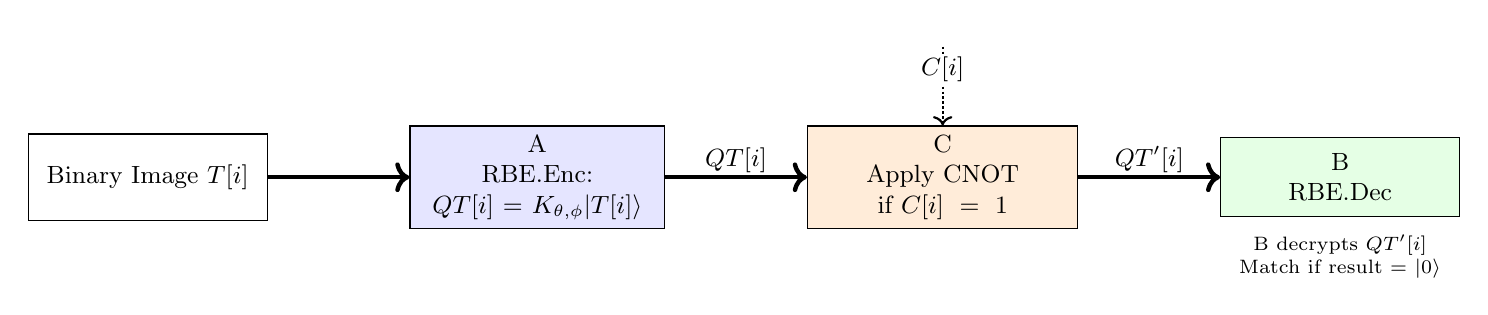
\begin{tikzpicture}[node distance=1.8cm and 1.8cm, font=\small]
  \tikzset{
    block/.style={rectangle, draw, minimum height=1.1cm, text width=2.8cm, align=center},
    roleA/.style={rectangle, draw, minimum height=1cm, text width=3.0cm, align=center, fill=blue!10},
    roleB/.style={rectangle, draw, minimum height=1cm, text width=2.8cm, align=center, fill=green!10},
    roleC/.style={rectangle, draw, minimum height=1cm, text width=3.2cm, align=center, fill=orange!15},
    arrow/.style={->, ultra thick},
    classical/.style={->, thick, densely dotted},
    labelabove/.style={midway, above, fill=white, inner sep=1pt},
  }

  % Nodes
  \node[block] (input) {Binary Image $T[i]$};
  \node[roleA, right=of input] (a) {A\\RBE.Enc:\\ $QT[i] = K_{\theta,\phi}|T[i]\rangle$};
  \node[roleC, right=of a] (c) {C\\Apply CNOT if $C[i] = 1$};
  \node[roleB, right=of c] (b) {B\\RBE.Dec};

  % Arrows
  \draw[arrow] (input) -- (a);
  \draw[arrow] (a) -- node[labelabove] {$QT[i]$} (c);
  \draw[arrow] (c) -- node[labelabove] {$QT'[i]$} (b);

  % Classical input to C
  \node[above=1.0cm of c] (cinput) {};
  \draw[classical] (cinput) -- node[labelabove] {$C[i]$} (c.north);

  % Match result label
  \node[below=0.1cm of b, font=\scriptsize, align=center] {
    B decrypts $QT'[i]$\\
    Match if result = $|0\rangle$
  };

\end{tikzpicture}
}
\caption{Distributed Quantum VES: A encrypts $T[i]$, C receives classical $C[i]$ and applies CNOT to $QT[i]$, B decrypts $QT'[i]$ to determine match.}
\label{fig:qves-final-flow}
\end{figure}

\newpage
\begin{lemma}
\label{lemma:match_zero}
Let $T[i], C[i] \in \{0,1\}$ be binary values representing the secret and candidate image pixels, respectively. Let $K_{\theta, \phi}$ be a unitary encryption key from the Random Basis Encryption (RBE) scheme. Define the encrypted qubit as:
\[
QT[i] = K_{\theta, \phi} \vert T[i] \rangle
\]
Let $QT'[i]$ be the transformed qubit after applying a CNOT gate conditioned on $C[i]$:
\[
QT'[i] = 
\begin{cases}
QT[i] & \text{if } C[i] = 0 \\
\text{CNOT}(QT[i]) & \text{if } C[i] = 1
\end{cases}
\]
Then, the decrypted result satisfies:
\[
\text{RBE.Dec}(QT'[i]) = 0 \iff T[i] = C[i]
\]
\end{lemma}

\begin{proof}
We analyze all possible values of $T[i]$ and $C[i]$:

\textbf{Step 1: Encryption.}  
The dealer encrypts $T[i] \in \{0,1\}$ using a secret unitary key:
\[
QT[i] = K_{\theta,\phi} \vert T[i] \rangle
\]

\textbf{Step 2: CNOT transformation (by C).}
\begin{itemize}
    \item If $C[i] = 0$, no gate is applied: $QT'[i] = QT[i] = K_{\theta,\phi} \vert T[i] \rangle$
    \item If $C[i] = 1$, a CNOT flips the bit: $QT'[i] = K_{\theta,\phi} \vert T[i] \oplus 1 \rangle$
\end{itemize}

\textbf{Step 3: Decryption (by B).}  
Participant B applies the inverse:
\[
K_{\theta,\phi}^{\dagger} QT'[i] = 
\begin{cases}
\vert T[i] \rangle & \text{if } C[i] = 0 \\
\vert T[i] \oplus 1 \rangle & \text{if } C[i] = 1
\end{cases}
\]
Measuring yields:
\[
\text{RBE.Dec}(QT'[i]) = T[i] \oplus C[i]
\]

\textbf{Conclusion.}  
Hence:
\[
\text{RBE.Dec}(QT'[i]) = 0 \iff T[i] = C[i]
\]

\textbf{Example.}  
Assume the original pixel is $T[i] = 1$ and the candidate is $C[i] = 1$:
\begin{itemize}
    \item A encrypts: $QT[i] = K_{\theta,\phi} \vert 1 \rangle$
    \item C applies CNOT: $\vert 1 \rangle \rightarrow \vert 0 \rangle$
    \item Result: $QT'[i] = K_{\theta,\phi} \vert 0 \rangle$
    \item B applies $K_{\theta,\phi}^{\dagger}$: $\vert 0 \rangle$
    \item Measures 0 $\Rightarrow$ Match confirmed
\end{itemize}

If instead $C[i] = 0$, CNOT is skipped, and B would decrypt back to $|1\rangle$, yielding result = 1 (a mismatch).

\end{proof}

\begin{center}
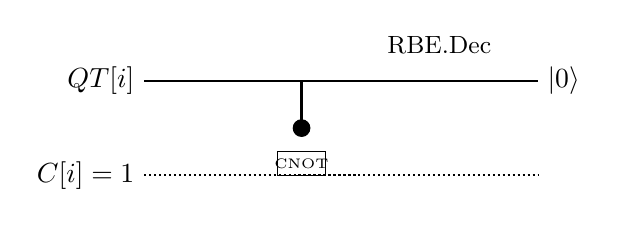
\begin{tikzpicture}
  \tikzset{
    operator/.style={draw, fill=blue!10, minimum size=1.0em},
    classical/.style={densely dotted, thick},
    wire/.style={thick},
  }

  % Qubit wire
  \draw[wire] (0,0) -- (5,0);
  \node[left] at (0,0) {$QT[i]$};

  % Classical wire
  \draw[classical] (0, -1.2) -- (5, -1.2);
  \node[left] at (0, -1.2) {$C[i] = 1$};

  % CNOT gate
  \draw[wire] (2,0) -- (2,-0.6);
  \filldraw[black] (2,-0.6) circle (3pt);
  \draw (1.7,-1.2) rectangle (2.3,-0.9);
  \node at (2,-1.05) {\tiny CNOT};

  % RBE.Dec label above wire
  \node at (3.75, 0.45) {\small RBE.Dec};

  % Output
  \node[right] at (5,0) {$|0\rangle$};

\end{tikzpicture}
\end{center}

% \section{QVES Resilient against Byzantine Participants}
% \label{qves_res_byzantine_part}
% Multiple C participants.
% A provides QT[i]_j multiple copies to C[j].
% Majority of C[j] determines C[i] image matching.
\section{QVES Resilient against Byzantine Participants}
\label{qves_res_byzantine_part}

To enhance robustness against faulty or malicious nodes, we extend the Quantum Visual Encryption Scheme (QVES) to support multiple $C$-type participants. This design enables the system to tolerate Byzantine behavior in the matching phase.

\subsection*{Architecture}

Let $A$ denote the encoder who performs RBE.Enc and generates the encrypted pixel qubit:
\[
QT[i] = K_{\theta_i,\phi_i} \vert T[i] \rangle
\]

Instead of sending $QT[i]$ to a single C participant, $A$ distributes \textbf{multiple copies} of the encrypted qubit:
\[
\{QT[i]_1, QT[i]_2, \dots, QT[i]_M\}
\]
to $M$ distinct C-type participants: $C[1], \dots, C[M]$.

Each $C[j]$ also receives the candidate image pixel value $C[i]$, and independently applies the conditional CNOT:
\[
QT'[i]_j =
\begin{cases}
QT[i]_j & \text{if } C[i] = 0 \\
\text{CNOT}(QT[i]_j) & \text{if } C[i] = 1
\end{cases}
\]

The architectude is shown on diagram \ref{fig:qves-byzantine}.

\subsection*{Decoding and Majority Vote}

Each transformed qubit $QT'[i]_j$ is forwarded to a B participant holding the decryption key $(\theta_i, \phi_i)$, who performs:
\[
\text{RBE.Dec}(QT'[i]_j) \in \{0,1\}
\]

All $M$ results are collected. If at least $\lceil M/2 \rceil$ participants agree that the decrypted value is $0$, then the system concludes:
\[
\texttt{Match}(T[i], C[i]) = \texttt{True}
\]

Otherwise, it is treated as a mismatch.

\subsection*{Byzantine Resilience}

This design tolerates up to $\lfloor (M - 1)/2 \rfloor$ Byzantine participants, under the assumption that:
- RBE.Dec cannot be faked without access to the correct $(\theta_i, \phi_i)$
- Each C[j] is independently provisioned and does not collude with others

\paragraph{Example.}
Suppose $M = 5$ and $T[i] = C[i] = 1$. Each C[j] receives a copy of $QT[i] = K_{\theta, \phi} |1\rangle$ and applies CNOT:
\[
QT'[i]_j = K_{\theta,\phi} |0\rangle
\]
Each B[j] decrypts:
\[
K_{\theta,\phi}^{\dagger} QT'[i]_j = |0\rangle \Rightarrow \texttt{Match}
\]
Even if two of the five participants return false results, the system concludes that the match holds.

\begin{figure}[ht]
\centering
\resizebox{\linewidth}{!}{
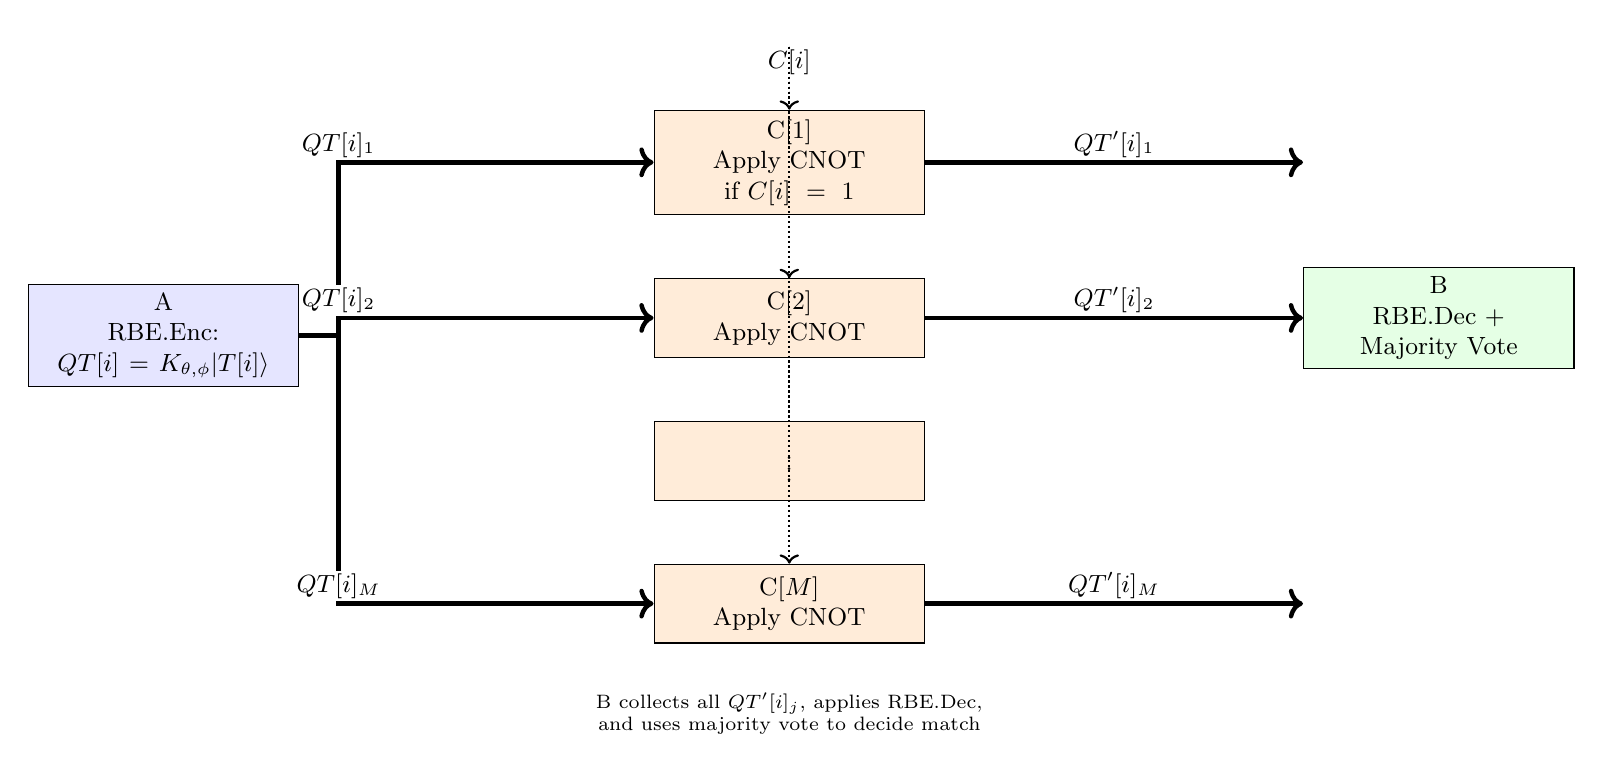
\begin{tikzpicture}[node distance=1.7cm and 1.7cm, font=\small]
  \tikzset{
    roleA/.style={rectangle, draw, minimum height=1cm, text width=3.2cm, align=center, fill=blue!10},
    roleB/.style={rectangle, draw, minimum height=1cm, text width=3.2cm, align=center, fill=green!10},
    roleC/.style={rectangle, draw, minimum height=1cm, text width=3.2cm, align=center, fill=orange!15},
    arrow/.style={->, ultra thick},
    classical/.style={->, thick, densely dotted},
    labelabove/.style={midway, above, fill=white, inner sep=1pt},
  }

  % Nodes
  \node[roleA] (a) {A\\RBE.Enc:\\ $QT[i] = K_{\theta,\phi}|T[i]\rangle$};

  \node[roleC, right=4.5cm of a, yshift=2.2cm] (c1) {C[1]\\Apply CNOT if $C[i] = 1$};
  \node[roleC, below=0.8cm of c1] (c2) {C[2]\\Apply CNOT};
  \node[roleC, below=0.8cm of c2] (c3) {$\vdots$};
  \node[roleC, below=0.8cm of c3] (cM) {C[$M$]\\Apply CNOT};

  \node[roleB, right=4.8cm of c2] (b) {B\\RBE.Dec +\\ Majority Vote};

  % A to Cs (qubit lines)
  \draw[arrow] (a.east) -- ++(0.5,0) |- node[labelabove] {$QT[i]_1$} (c1.west);
  \draw[arrow] (a.east) -- ++(0.5,0) |- node[labelabove] {$QT[i]_2$} (c2.west);
  \draw[arrow] (a.east) -- ++(0.5,0) |- node[labelabove] {$QT[i]_M$} (cM.west);

  % Classical control line to Cs
  \node[above=0.8cm of c1] (ctrl) {};
  \draw[classical] (ctrl) -- node[labelabove] {$C[i]$} (c1.north);
  \draw[classical] (ctrl) -- (c2.north);
  \draw[classical] (ctrl) -- (cM.north);

  % Cs to B
  \draw[arrow] (c1.east) -- node[labelabove] {$QT'[i]_1$} (b.west |- c1.east);
  \draw[arrow] (c2.east) -- node[labelabove] {$QT'[i]_2$} (b.west |- c2.east);
  \draw[arrow] (cM.east) -- node[labelabove] {$QT'[i]_M$} (b.west |- cM.east);

  % Description box below
  \node[below=0.5cm of cM, font=\scriptsize, align=center] {
    B collects all $QT'[i]_j$, applies RBE.Dec,\\
    and uses majority vote to decide match
  };

\end{tikzpicture}
}
\caption{Byzantine-resilient QVES architecture: A sends $QT[i]$ to multiple C participants, each applies conditional CNOT, and B aggregates their transformed qubits for majority-decision decryption.}
\label{fig:qves-byzantine}
\end{figure}

\section{Multiple Matches Support}
To support matching against multiple candidate images \\ \( C_1, C_2, \ldots, C_k \), we must prepare multiple copies of the encrypted quantum state \( QT[i] = K_{\theta_i, \phi_i} \vert T[i] \rangle \) for each pixel \( i \). This is necessary because each comparison consumes a unique quantum copy — due to the destructive nature of quantum measurement and the constraints of the No-Cloning Theorem~\cite{wootters1982nocloning}.

Formally, for \( k \) independent candidate images, we require \( k \) copies of each pixel qubit to evaluate the match:
\[
\{ QT[i]_1, QT[i]_2, \ldots, QT[i]_k \}
\]
Each copy is used exactly once for matching against a corresponding \( C_j[i] \), and cannot be reused. This ensures both correctness and information-theoretic security in the multi-match setting.

\section{Security Model Analysis}
\label{sec_model_analysis}

% \section{Collaborative Secure Image Matching}
% \label{collaborative_secure_images_matching}

% First, the participant acquires a candidate image $C$. For each pixel $C[i]$ of the image, if the pixel is \textbf{black}, the participant computes the Kronecker product with $D$ as
% \[
% QT_d[i] = QT[i] \otimes D,
% \]
% thus transforming the original $T[i]$ value. 

% The gate $D$ operates as follows:
% \[
% T[i] =
% \begin{cases}
% \text{white} &\Rightarrow\  QT_d[i] \ \text{is black},\\
% \text{black} &\Rightarrow\  QT_d[i] \ \text{is white}.
% \end{cases}
% \]

% During the computation, participants do not observe the state of either $QT[i]$ or $QT_d[i]$, so the original pixel value of $T[i]$ remains unknown to them at all times. 

% Afterwards, the participants transmit $QT_d[i]$ to the dealer, who reads its state. If $QT_d[i]$ is \textbf{black}, it follows that $T[i]$ and $C[i]$ do not match; if $QT_d[i]$ is \textbf{white}, then $T[i]$ and $C[i]$ match.


% In our previous paper \cite{10013507}, we examined the Collaborative Secure Images Matching problem. The problem is defined as follows: There is a secret image and a set of $n$ mobile agents. The mobile agents need to match (or compare) an observed image to the original secret image. Importantly, during the matching process secret image should be hidden, thus no information about the original image should be disclosed. We previously discussed applications of the Collaborative Secure Images Matching solution, including its use in UAV swarms. Similarly, the Waves Interference VES-based solution is well-suited for the UAV swarm scenario.
% The proposed solution is based on the well-known Visual Encryption Scheme (VES) and projections of visual bit maps rather than (quadratic complexity) messages exchange in implementing Secure Multi Party Computation (MPC) scheme. We proved that the proposed solution is perfect-information-theoretic secure. To retrieve any information about the original image, at least $d$ out of $n$ mobile agents are required.
% Similarly, we present Collaborative Secure Images Matching solution based on the proposed in Section \ref{chapter:our_solution} Waves Interference based Visual Encryption Scheme.

% \subsection{Collaborative Secure Images Matching Solution}
% \label{collaborative_secure_images_matching_solution}
% As in the solution proposed in the paper \cite{10013507}, in the Waves Interference VES-based solution, the secret image is encrypted using a VES scheme with a threshold $d \leq n$. Each mobile agent $P_i$ is assigned a share $T_i$ of the secret image. Agents that acquire the candidate image and intend to match it to the secret image do not reconstruct the secret image from the VES shares. Instead, agents perform two possessed share (wave) transmissions to the counting device for white and black pixel matching, as described below. Finally, the counting device makes the images' matching decision.

% Assumptions. All swarm participants acquire the same candidate image and are synchronized. This means that they acquire the same candidate image $C$.

\section{Color Images Support}
\label{chapter:color_images_support}
% The Waves Interference based VES solution can be easily extended to support grey scale and color images. As in in the paper \cite{10013507}, Discrete Bits as Pixels or Unary Mapping Step Function approaches can be applied in the same way - on beams representing the information bits.

\section{Comparative Analysis}
\label{chapter:comparative_analysis}


%\textcolor{blue}{
\section{Experiments}
\label{chapter:experiments}

\section{Conclusions and Future Directions}
\label{chapter:discussion_and_conclusions}

% This paper presents a Visual Encryption Scheme (VES) based on the physical phenomenon of wave interference. The proposed scheme addresses the well-known monotonicity problem and enables the use of perfect black-and-white or color pixels in both the VES shares and the reconstructed image. Furthermore, leveraging wave interference improves the security model by introducing resilience against active Byzantine adversaries.

% The architectural reference for implementing the Wave Interference-based VES is outlined in Section~\ref{chapter:our_solution}. As demonstrated in Section 4, the use of wave interference ensures not only statistically information-theoretic security against honest-but-curious adversaries, but also robustness against active adversaries attempting to disrupt the system.

% The proposed scheme is applicable to the Collaborative Secure Image Matching problem, discussed in Section~\ref{collaborative_secure_images_matching}. Both grayscale and color images can be effectively handled, as shown in Section~\ref{chapter:color_images_support}. Experiments demonstrating the effectiveness of the Wave Interference-based VES are detailed in Section~\ref{chapter:experiments}.

% Future research directions include:
% \begin{itemize}
%     \item Exploring the application of Wave Interference VES in video steganography frameworks, such as those discussed in~\cite{LIU2019238, LIU201663}, where the use of discrete pixel-level encoding aligns naturally with video frame structures.
%     \item Investigating the scheme's resilience to crash failures within a swarm of participants—particularly scenarios where only a subset of the shares are available during reconstruction.
%     \item Analyzing performance trade-offs between optical implementation fidelity, interference precision, and practical hardware deployment.
% \end{itemize}

\section*{Acknowledgments}
This research was (partially) funded by the Israeli Science Foundation (Grant No. 465/22) and by the Army Research Office under Grant
Number W911NF-22-1-0225, and by Rita Altura trust chair in computer science. The views and conclusions contained in this document are those of the authors and
should not be interpreted as representing the official policies, either expressed or implied, of the Army Research Office or the U.S. Government. The U.S. Government is authorized to reproduce and distribute reprints for
Government purposes notwithstanding any copyright notation herein.
\section*{Declarations}
\noindent{\bf Conflict of interest} The authors do not have any conflict of interest in hiring, financial support, or others. \\
{\bf Data availability statement} Our manuscript does not have associated data.

%\listoffigures
%\listoftables

%\bibliographystyle{plain}
%\bibliographystyle{alpha}
%\bibliographystyle{splncs04}
\bibliographystyle{elsarticle-num}
%\bibliographystyle{elsarticle-harv}

\bibliography{thesis}
\end{document}
